\chapter{Simulation et Réalisation}
\section{Conception du logiciel}
\subsection{Description détaillée de la conception du logiciel}
\subsubsection{Architecture logicielle}
Ce système (SRI) est un système orienté WEB utilisant l'architecture MVC ou Modèle Vue Controlleur. C'est un motif d'architecture logicielle destiné aux interfaces graphiques, lancé en 1978 et très populaire pour les applications web \citep{mvcwiki}.

Cet architecture est illustré dans la Figure~\ref{fig:mvc}

\begin{figure}[htbp]
    \begin{center}
        \fbox{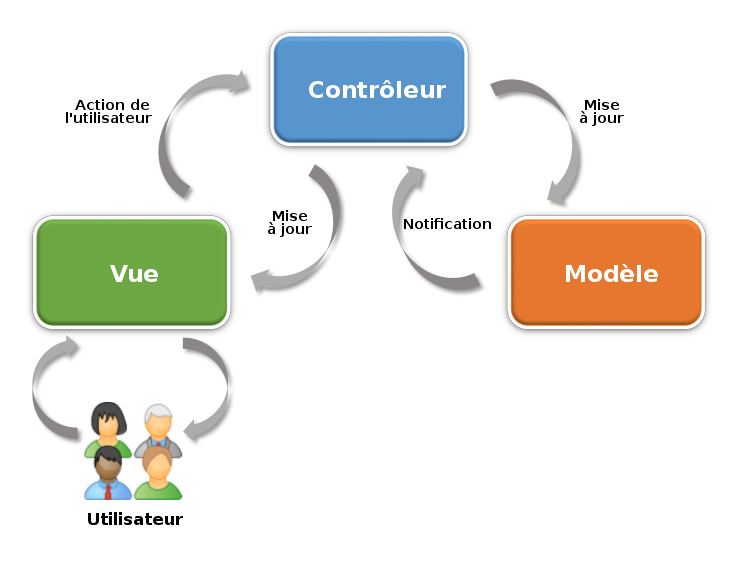
\includegraphics[width=13cm, angle=0]{Figures/Realisation/mvc.png}}
    \end{center}
    \caption{Architecture MVC \citep{mvcwiki}}\label{fig:mvc}
\end{figure}

\subsubsubsection*{Le Modèle (Model)}
Le Modèle contient les données a afficher a l'utilisateur. En d'autre terme, c'est la representation de la base de données. Dans le cadre de ce système, l'index inversé, les documents ainsi que les catégorie des documents sont representé par un modèle chacun.

\subsubsubsection*{La Vue (View)}
Elle contient la representation graphique, tel que les formulaires, les listes, les tables, etc. Elle est généralement ecrite en langage HTML pour une application WEB\@. Elle represente la formulaire de recherche, ainsi que les différenes filtres de recherche par l'utilisateur, et aussi les parties concernant l'authentification et d'autres.

\subsubsubsection*{Le Controlleur (Controller)}
Il contient la logique concernant les actions effectuées par l'utilisateur. En d'autre terme, il est le chef d'orchestre du système, traite les informations provenant de l'utilisateur et les persister dans la base de données et de recuperer des données et de les afficher a l'utilisateur. Dans ce système, il est responsable de tous traitement de documents, authentification, et d'autres traitements comme le telechargement et protection des documents.

Il est utilisé par de nombreux frameworks pour applications web tels que Ruby on Rails, Grails, ASP.NET MVC, Spring, Struts, Symfony, Apache Tapestry, Laravel, AdonisJS, Django ou AngularJS\@.

\subsubsection{Choix de conception clés}
Pour ce système, on distingue deux type de conception tel que la \emph{conception de la base de données} et la \emph{conception de l'interface utilisateur}. Pour la base de données, deux approche sont possible tel que \emph{MERISE} et \emph{UML}. L'une de grande différence entre MERISE et UML ce que MERISE traite les données et les traitements séparement tandis que UML non.

\subsubsubsection*{MERISE}
Merise est une méthode informatique dédiée à la modélisation qui analyse la structure à informatiser en terme de systèmes. Le gros avantage de cette méthode est qu’elle permet de cadrer le projet informatique et de \emph{discuter} en se comprenant entre utilisateurs et informaticiens \citep*{base-de-donnees}.

Créée dans les années 70 sur commande de l’État français et destinée aux gros projets informatiques de l’époque, la méthode a perduré jusqu’à aujourd’hui. Son utilisation très répandue en Europe constitue un socle difficilement contournable lorsque l’on s’attache à la création de bases de données.

Merise est en fait un outil analytique qui facilite la création de base de données et de projets informatique. Le principal auteur de la méthode est Hubert Tardieu qui se basa sur les travaux autour du modèle relationnel de Codd.

Elle permet réelement de:
\begin{itemize}
    \item décrire le fonctionnement du système à informatiser tel que les \textbf{données} representé par le MCD (Modèle Conceptuel de Données) qui determine les relations et les dépendances entres les différents acteurs (utilisateur, administrateur, documents), et les \emph{traitements} representé par le MCT (Modèle Conceptuel de Traitement) qui determine comment les acteurs travaillent-ils ensemble.
    \item proposer une implémentation logique tel que MLD (Modèle Logique de Données), MLT (Modèle Logique de Traitement).
    \item Proposer une construction concrète et utilisable du point précédent tel que la MPD (Modèle Physique de Donnée).
\end{itemize}

\subsubsubsection*{UML}
Le Langage de Modélisation Unifié, de l'anglais Unified Modeling Language, est un langage de modélisation graphique à base de pictogrammes conçu comme une méthode normalisée de visualisation dans les domaines du développement logiciel et en conception orientée objet. L'UML est une synthèse de langages de modélisation objet antérieurs: Booch, OMT, OOSE \citep*{UMLorg}.

Principalement issu des travaux de Grady Booch, James Rumbaugh et Ivar Jacobson, UML est à présent un standard adopté par l'Object Management Group. UML 1.0 a été normalisé en janvier 1997; UML 2.0 a été adopté par l'OMG en juillet 2005.

UML propose différentes diagrammes, et principalement catégorisé en trois catégories:
Bien sûr, voici une explication détaillée de chaque catégorie de diagrammes UML :

\begin{enumerate}
    \item \textbf{Structure}: Où on trouve
    \begin{itemize}
        \item \emph{Diagramme de classes}: Il montre la structure statique d'un système en mettant l'accent sur les classes du système, leurs attributs, leurs opérations et les relations entre les classes.
        \item \emph{Diagramme d'objets}: Il illustre des exemples spécifiques d'objets et de relations entre ces objets, montrant une instance particulière d'un diagramme de classes à un moment donné.
        \item \emph{Diagramme de composants}: Il met l'accent sur les composants d'un système logiciel et leurs dépendances, en montrant la structure des composants et la manière dont ils interagissent au niveau de l'architecture.
        \item \emph{Diagramme de paquetages}: Il organise les éléments d'un modèle en groupes, montrant comment ces éléments sont regroupés en paquets et les relations entre les paquets.
    \end{itemize}
    \item Comportément
    \begin{itemize}
        \item Diagramme de cas d'utilisation: Il décrit les interactions entre les utilisateurs et un système donné, mettant l'accent sur les fonctionnalités offertes par le système du point de vue de l'utilisateur.
        \item Diagramme de séquence: Il montre l'interaction entre les objets, en mettant l'accent sur la séquence temporelle des messages échangés entre les objets lors de l'exécution d'un scénario particulier.
        \item Diagramme d'activités: Il représente le flux de contrôle d'une activité ou d'un processus, mettant l'accent sur les actions et les décisions qui composent le processus.
        \item Diagramme d'états-transitions: Il modélise les transitions d'états pour un objet ou une entité donnée, montrant comment l'objet réagit aux événements au fil du temps.
    \end{itemize}
    \item Déploiement
    \begin{itemize}
        \item Diagramme de déploiement: Il montre la configuration matérielle d'un système et la manière dont les composants logiciels sont déployés sur cette configuration matérielle.
    \end{itemize}
\end{enumerate}

Ces différentes catégories de diagrammes UML offrent des moyens visuels efficaces pour modéliser les différents aspects d'un système logiciel, ce qui facilite la compréhension et la communication entre les différentes parties prenantes impliquées dans le processus de développement logiciel.

Dans le cadre de ce dévoir, on utilisera l'approche UML, vu qu'on utilise une architecture MVC et une approche orienté objet (OOP), cette approche sera plus bénéfique. Mais il est possible et ce sera envisageable d'utiliser Merise pour ce système.

Pour la conception de l'interface utilisateur, le langage de balisage HTML5, le feulle de style CSS3 ainsi que le langage JavaScript est utilisé.

\subsubsubsection*{SGBD}
Un SGBD ou Système de Gestion de Base de Données est un logiciel système permettant aux utilisateurs et programmeurs de créer et de gérer des bases de données. Plus précisement, il permet a un ordinateur de stocker, récupérer,
ajouter, supprimer et modifier des données. Ce système est aujourd’hui utilisé dans presque tous les outils que nous utilisons \citep*{oracleDB}.

Le SGBD gère trois choses importantes: les \emph{données}, le \emph{moteur de base de données} qui permet d'accéder aux données, de les verrouiller et de les modifier, et le \emph{schéma de base de données}, qui définit la structure logique de la base de données. Ces trois éléments fondamentaux contribuent à assurer la concomitance, la sécurité, l'intégrité des données et l'uniformité des procédures administratives \citep*{oracleDB}.

\subsubsection{Les fonctionnalités de base}
Citons les fonctionnalités de base qui sont le plus importants pour ce système.
\begin{enumerate}
    \item \textbf{Indexer des documents}: capacité d'indexer des documents textuelles de différente format tel que PDF, WORD et peut être des images donténant des textes. Cette fonctionnalité inclus l'extraction automatique de titre, resumé, date de soutenance, ainsi de faire un traitement de langage naturel. Cette donctionnalité se fait par un upload de fichier dans un navigateur WEB\@.
    \item \textbf{Système d'authentification}: permet a l'utilisateur de s'authentifier ou se créer des comptes afin de deposer et telecharger des documents. Elle permet aussi aux amdinistrateurs de valider des documents, les supprimer si necessaire. Elle permet aussi de disposer d'un espace membre en tant qu'étudiant et en tant qu'enseignant, verouller des documents et de ne donner l'accès qu'a certains utilisateurs.
    \item \textbf{Recherche par mots clés}: ette fonctionnalité permet aux utilisateurs de faire des recherches en utilisant une zone de saisie par des mots clés afin de satisfaire ses besoins. Cette fonctionnalité inclus d'autres fonctionnalités tel que le \emph{système de filtre de recherche}: recherche par conténu, par titre ou par auteur; \emph{système de filtre d'organisation}: par année croissante ou décroissante, par université; \emph{traitement de la reqête}: suppréssion des mots vides, correction des orthographes, pondération du terme de la requête. Elle se charge de faire l'appariément entre la requête de l'utilisateur et les documents dans la collection, et afficher ensuite les résultats par ordre de pertinence décroissante. L'utilisateur peut avoir une suggestion des mots clés lorsqu'il exprime son besoin d'information.
    \item \textbf{Page de resultat et visualisation de document}: permet d'afficher les resultats avec des paginations, ainsi que la possibilité de visualiser le resumé ou la partie du document. Il est aussi possible de visualiser un document en entier.
\end{enumerate}

\subsection{Technologies et outils utilisés}
\subsubsection{Technologies}
Pour develloper ce SRI, on a utilisé des téchnologies orientés vers l'intelligence artificiel implementé dans un application web. On aura utilisé une base de données pour stocker les données tel que les documents, les informations de l'utilisateur, etc. Ci-dessous la liste des téchnologies utilisés pour la réalisation de ce système.

\begin{itemize}
    \item \textbf{Framework Django}: est un framework web developpé en langage Python tilisant l'architecture MVT (Model-View-Template). A bien noter que dans Django, View est l'equivalent d'un Controlleur et que Template est l'equivalent de Vue. Ce choix est dû au fait qu'il est facile d'integré des librairies d'intelligence artificiel dans ce framework, ainsi que les fonctionnalités pré-concus facilitera beaucoup le devellopement \citep*{django}.
    \item \textbf{MySQL}: pour stocker les données comme on a dit ci-dessus. Elle est gratuite et largement suffisant pour ce genre de système en terme de capacité de stockage et en terme de rapidité de récuperation des données \citep*{mysql}.
    \item \textbf{Spacy}: est un librairy python permettant de faire un traitement de langage naturel. Il utilise un modèle de machine learning pré-entrainé pour différentes langages. Comme pour la langue française par exemple il y a les modèle \emph{frcorewebnewssm}. Ce librairie permet de segmenter des textes en français, supprimer les mots vides, et recupérer la racine des mots, c'est ce librairie qui se charge de l'indexation dans ce SRI \citep*{spacy}.
    \item \textbf{NLTK}: ou Natural Language Toolkit est aussi ule librairie de traitement de langage naturel \citep*{nltk}
    \item Numpy \citep*{numpy}
    \item ScikitLearn \citep*{scikit-learn}
    \item PDFPlumber \citep*{pdfplumber}
    \item FItz library \citep*{fitz}
    \item Spellchecker library \citep*{spellchecker}
\end{itemize}

\subsubsection{Langage de programmation}
Description des langages de programmation utilisés pour la mise en œuvre du logiciel, par exemple, Python, Java, ou JavaScript. Justification de l'utilisation de ces langages en fonction de leur adaptabilité aux exigences spécifiques du logiciel.

\begin{itemize}
    \item Python \citep*{python}
    \item SQL
\end{itemize}

\subsubsection{Outils}
Présentation des outils de développement utilisés, comme les environnements de développement intégrés (IDE), les systèmes de contrôle de version, et les outils de test. Explication de la façon dont ces outils ont facilité le processus de conception et de développement du logiciel.

\begin{itemize}
    \item Visual Studio Code (Explication de ses diverses extensions) \citep*{vscode}
    \item Git et Github (Système de controle de version / Explication de la facilité de suivre des modifications) \citep*{git, github}
    \item Machine utilisé pour le développement (CPU, GPU, RAM, HDD, OS)
    \item Outil de test de django
\end{itemize}

\section{Développement du logiciel}
\subsection{Présentation des différentes étapes du processus de développement}
\subsubsection{Planification}
Explication du processus de planification, y compris l'identification des fonctionnalités clés, la répartition des tâches et la définition des jalons du projet. Discussion sur la manière dont la planification a facilité le développement du logiciel.

\subsubsection{Programmation}
Description des étapes de programmation, y compris la mise en œuvre des fonctionnalités principales du logiciel et la résolution des problèmes techniques rencontrés lors du processus de développement. Illustration de certains segments de code pertinents pour la compréhension du développement.

\subsubsection{Tests}
Présentation de la stratégie de test adoptée pour évaluer le bon fonctionnement du logiciel. Description des tests unitaires, des tests d'intégration et des tests de validation effectués pour assurer la qualité du logiciel.

\subsection{Défis rencontrés lors du développement et solutions mises en œuvre}
\subsubsection{Contraintes techniques}
Discussion sur les problèmes techniques spécifiques rencontrés lors du développement et des solutions techniques mises en place pour les surmonter. Analyse des obstacles et des stratégies d'atténuation adoptées pour assurer la progression continue du projet.

\subsubsection{Gestion des délais}
Évaluation des défis liés à la gestion du temps et des échéances du projet. Présentation des techniques de gestion de projet mises en place pour respecter les délais et assurer la livraison du logiciel dans les délais impartis.

\subsubsection{Collaboration d'équipe}
Discussion sur les enjeux liés à la collaboration au sein de l'équipe de développement et des mesures prises pour favoriser une communication efficace et une coordination harmonieuse entre les membres de l'équipe.

\section{Tests et validation du logiciel}
\subsection{Stratégies de test utilisées pour évaluer la performance et la fonctionnalité du logiciel}
\subsubsection{Tests unitaires}
Description des tests unitaires réalisés pour vérifier le bon fonctionnement des composants individuels du logiciel.

\subsubsection{Tests d'intégration}
Présentation des tests d'intégration effectués pour évaluer l'interopérabilité des différents modules du logiciel.

\subsubsection{Tests de validation}
Explication des tests de validation effectués pour vérifier si le logiciel répond aux exigences spécifiées dans le cahier des charges.

\subsection{Résultats des tests et analyse critique des performances du logiciel}
\subsubsection{Résultats des tests}
Présentation des résultats détaillés des tests effectués, y compris les rapports de tests, les captures d'écran et les données de performance.

\subsubsection{Identification des problèmes}
Discussion sur les éventuels problèmes ou erreurs identifiés au cours des tests, avec analyse critique des mesures prises pour corriger ces problèmes.

\section{Implémentation du logiciel dans un contexte réel}
\subsection{Processus d'implémentation}
Explication du processus d'implémentation du logiciel dans un environnement réel, en mettant l'accent sur les étapes clés et les considérations spécifiques prises en compte lors du déploiement.

\subsection{Évaluation de l'efficacité de l'implémentation}
Analyse de l'efficacité de l'implémentation du logiciel en fonction des objectifs initiaux et des résultats observés dans le contexte réel.

\subsection{Rétroaction des utilisateurs}
Présentation des retours d'expérience et des commentaires des utilisateurs finaux concernant l'utilisation et les performances du logiciel dans leur environnement réel.

\subsection{Réponses aux problèmes éventuels}
Discussion sur la manière dont les problèmes éventuels rencontrés lors de l'implémentation ont été résolus, et sur les ajustements apportés pour améliorer l'expérience utilisateur et les performances du logiciel.

\section{Évaluation des performances et des résultats}
\subsection{Évaluation critique des performances du logiciel}
Analyse approfondie des performances du logiciel en termes de fonctionnalité, de convivialité, de fiabilité et d'efficacité, en se référant aux critères établis au début du projet.

\subsection{Comparaison avec les objectifs initiaux}
Comparaison des performances réelles du logiciel avec les objectifs initiaux définis lors de la conception, en mettant en évidence les écarts éventuels et les facteurs contributifs.

\subsection{Identification des forces et des faiblesses}
Identification des points forts et des limitations du logiciel en fonction des retours d'expérience des utilisateurs et des évaluations techniques, en mettant l'accent sur les domaines nécessitant d'éventuelles améliorations ou ajustements.

\subsection{Implications et recommandations}
Discussion des implications des résultats obtenus, avec des recommandations pratiques pour l'amélioration continue du logiciel ainsi que des suggestions pour des développements futurs ou des extensions potentielles.

\section{Réflexions sur l'expérience de développement}
\subsection{Analyse critique des leçons apprises}
Analyse réfléchie des principaux enseignements tirés de l'expérience de développement du logiciel, en mettant l'accent sur les succès, les défis et les stratégies d'adaptation ou d'amélioration.

\subsection{Évaluation de l'efficacité des stratégies de développement}
Évaluation de l'efficacité des différentes stratégies de développement utilisées tout au long du processus, en mettant en évidence les approches qui ont bien fonctionné et celles qui auraient pu être améliorées.

\subsection{Suggestions pour des améliorations futures}
Proposition de suggestions concrètes pour améliorer les processus de développement, les stratégies de gestion de projet et les approches techniques pour de futurs projets similaires.

\subsection{Perspectives de recherche future}
Discussion sur les pistes de recherche future potentielles basées sur les lacunes identifiées dans le cadre du projet actuel, en mettant l'accent sur les domaines qui méritent une exploration plus approfondie et des développements ultérieurs.